%%%%%%%%%%%%%%%%%%%%%%%%%%%%%%%%%%%%%%%%%%%%%%%%%%%%%%%%%%%%%%%%%%%%%%%
%% Document: Thesis for PhD at UC Riverside                          %%
%% Description: A comparative analysis of environment sensing in EDF %%
%% Author: Steven Ahrendt                                            %%
%%%%%%%%%%%%%%%%%%%%%%%%%%%%%%%%%%%%%%%%%%%%%%%%%%%%%%%%%%%%%%%%%%%%%%%
% COELOMOMYCES FIGURES %
%%%%%%%%%%%%%%%%%%%%%%%%
\begin{figure}[hb]
  \centering
  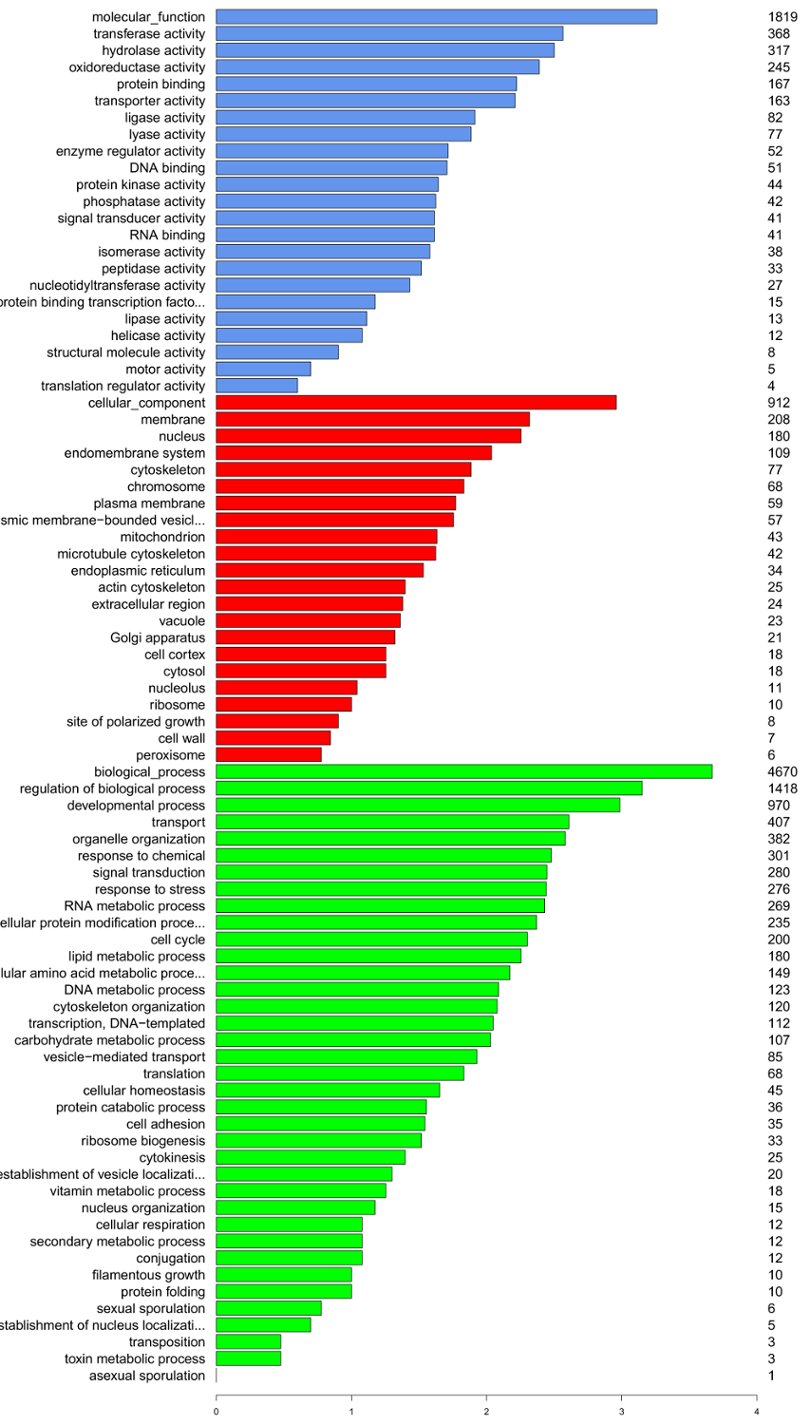
\includegraphics[width=4in]{./Chapter_Coelomomyces/img/Clat_aspergillus_GOPlot.png}
  \caption[Distribution of \textit{Aspergillus} GO-Slim terms associated with \textit{C. lat} transcriptome.]{Horizontal bar chart showing the distribution of \textit{Aspergillus} GO-Slim terms associated with the \textit{C. lat} transcriptome. X axis is a logarithmic scale.}
  \label{fig:ChClat_GOPlot}
\end{figure}
\begin{figure}[hb]
  \centering
  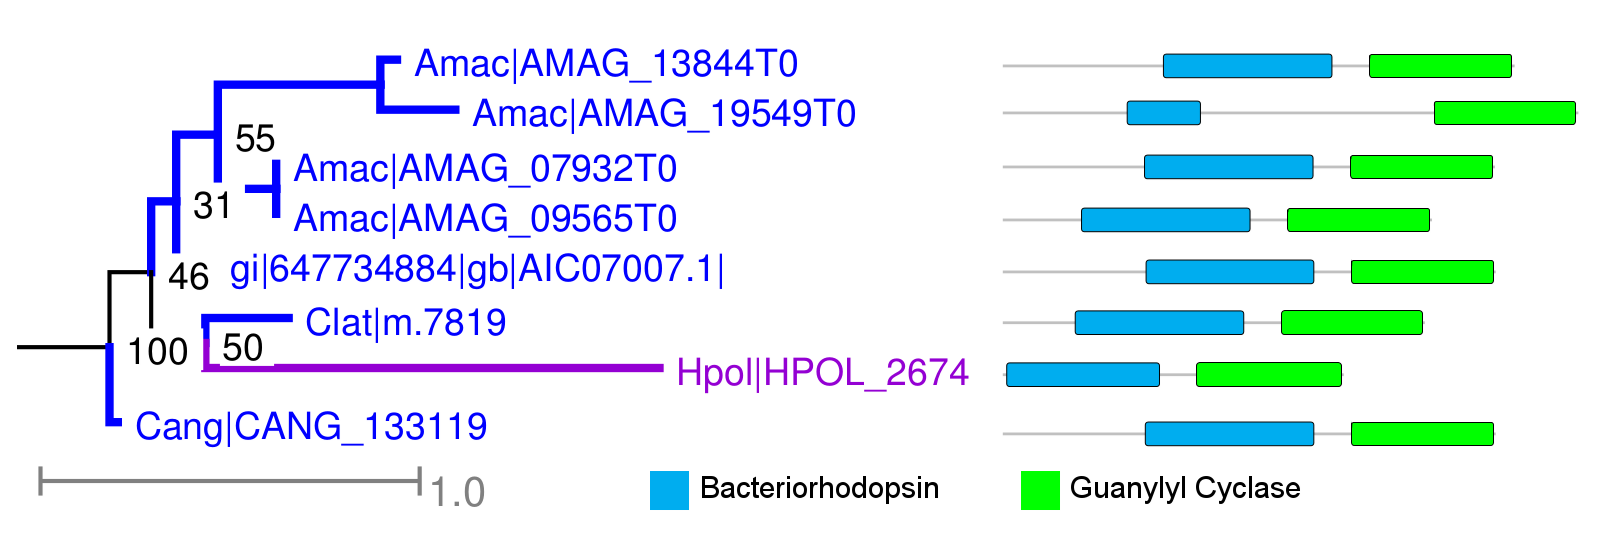
\includegraphics[width=4in]{./Chapter_Coelomomyces/img/OpsinGCFusion_chytridCluster.png}
  \caption[Opsin-GC fusion proteins; Chytridiomycota and Blastocladiomycota cluster]{A subset of opsin}
  \label{fig:ChClat_OpsinGC}
\end{figure}
\begin{figure}[hb]
  \centering
  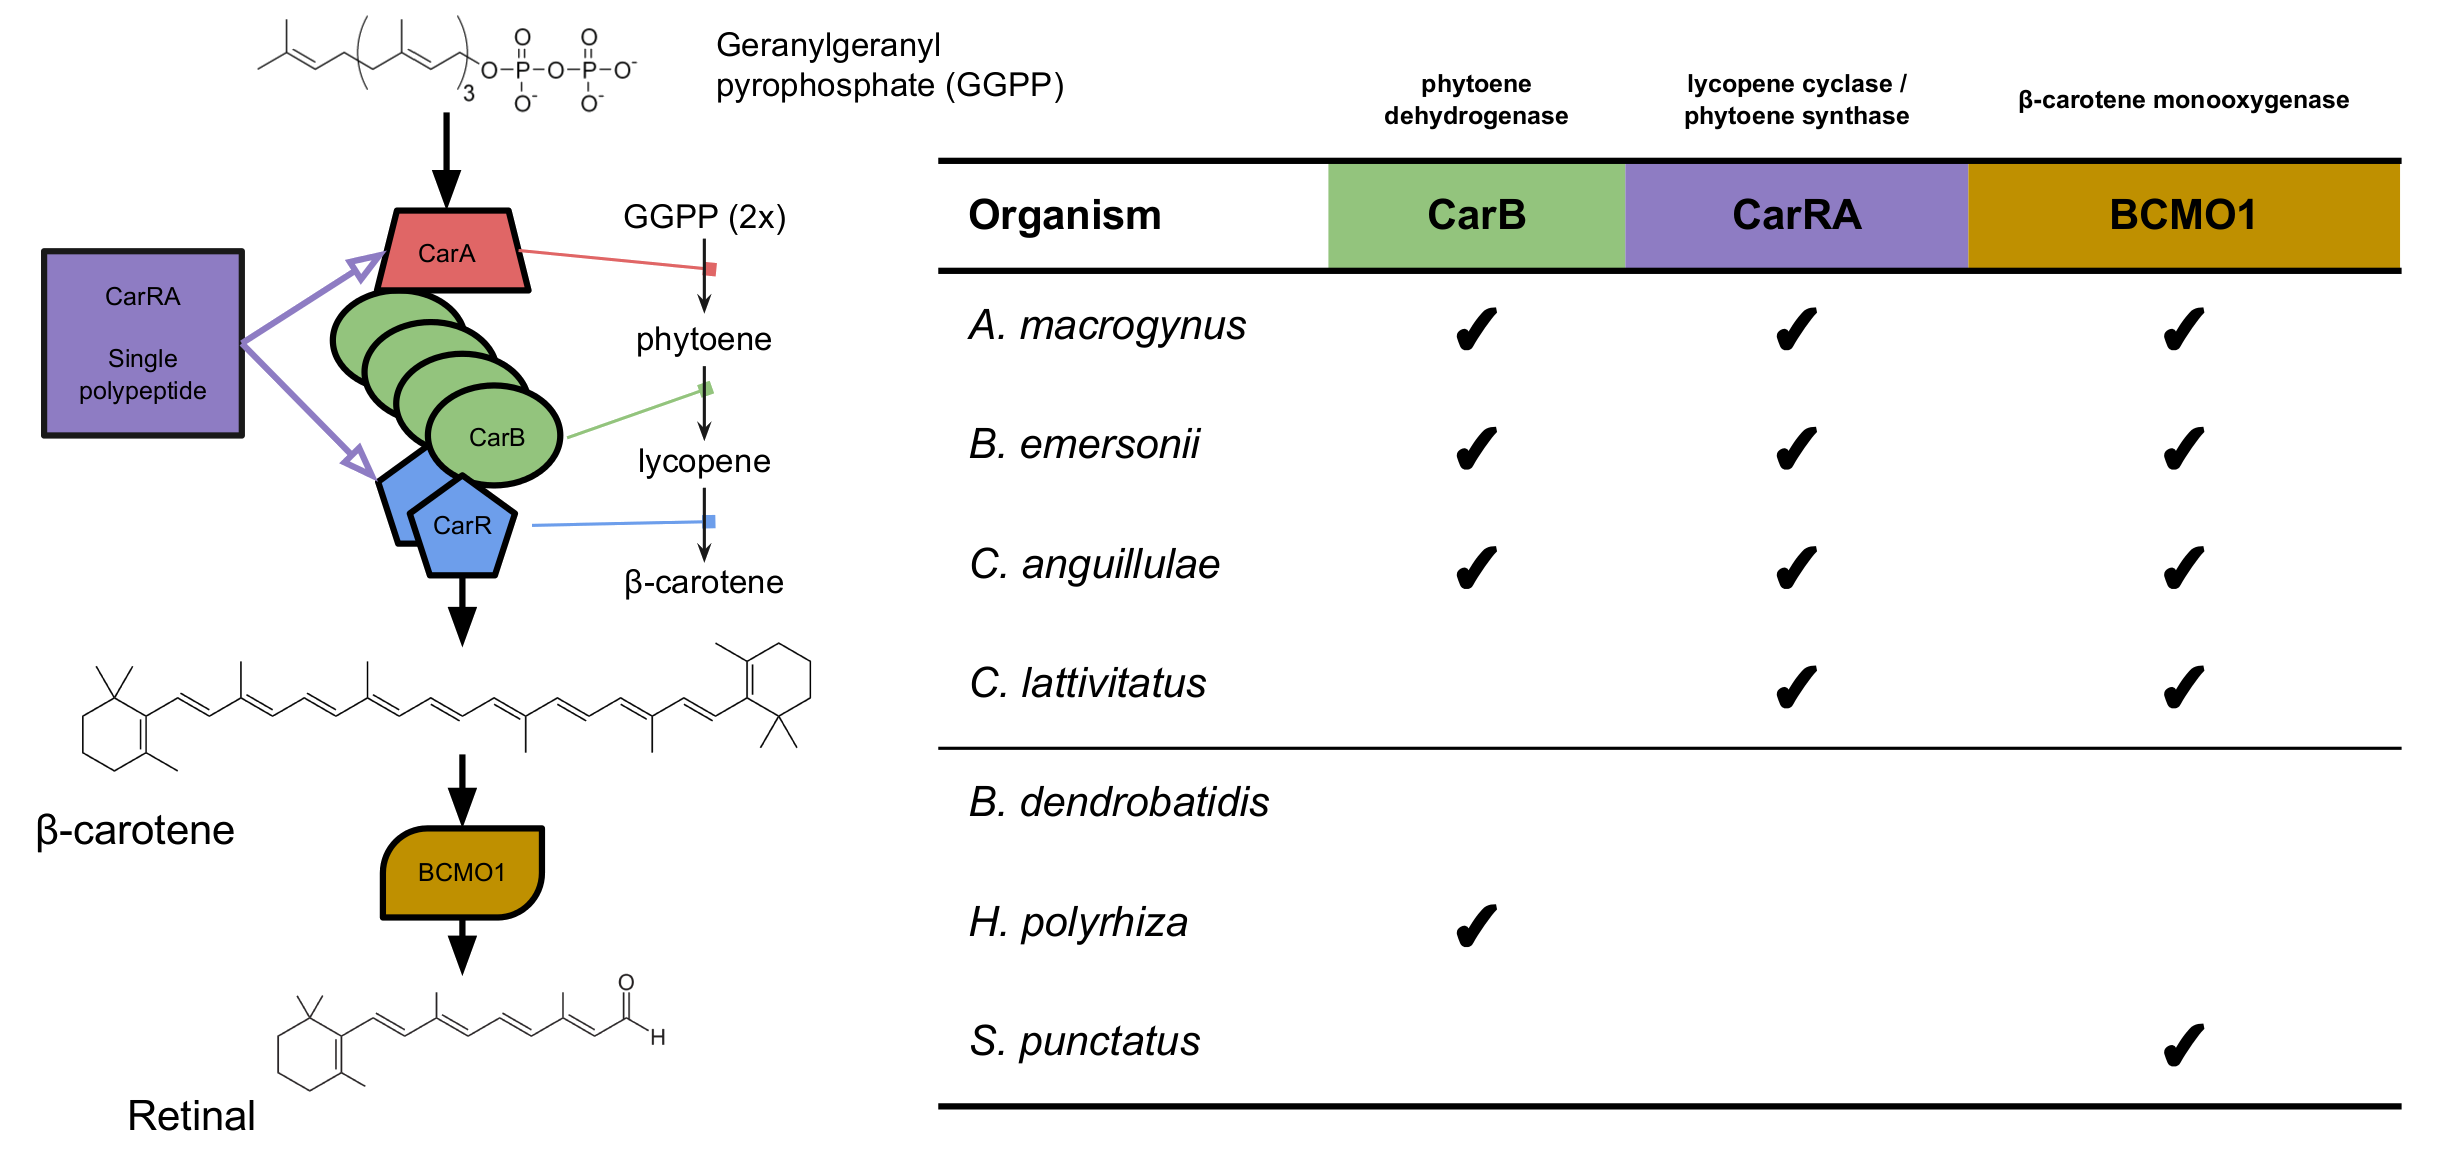
\includegraphics[width=4in]{./Chapter_Coelomomyces/img/Figure_bcaroPresenceAbsence.png}
  \caption[$\beta$-carotene enzyme presence / absence]{Presence and absence of $\beta$-carotene related proteins in species belonging to the Chytridiomycota and Blastocladiomycota.}
  \label{fig:ChClat_Bcaro}
\end{figure}
%\begin{figure}[hb]
%  \centering
%  \includegraphics[width=4in]{}
%  \caption[Maximum likelihood tree for PF00112 Cysteine protease proteins in \textit{C. lat} and others.]{RAxML tree of PFAM seed sequences, unique \textit{C. lat} protein sequences, and eight sequences with this domain from six Dikarya species: five ascomycetes (\textit{Thielavia heterothallica}, \textit{Thielavia terrestris}, \textit{Chaetomium globosum}, \textit{Podospora anserina}, and \textit{Hypocrea atroviridis}) and one basidiomycete (\textit{Laccaria bicolor}).}
%  \label{fig:ChClat_PF00112}
%\end{figure}
